\documentclass[tikz]{standalone}
\usepackage{pgfplots}
\usetikzlibrary{intersections}
\pgfplotsset{compat=1.17}
\begin{document}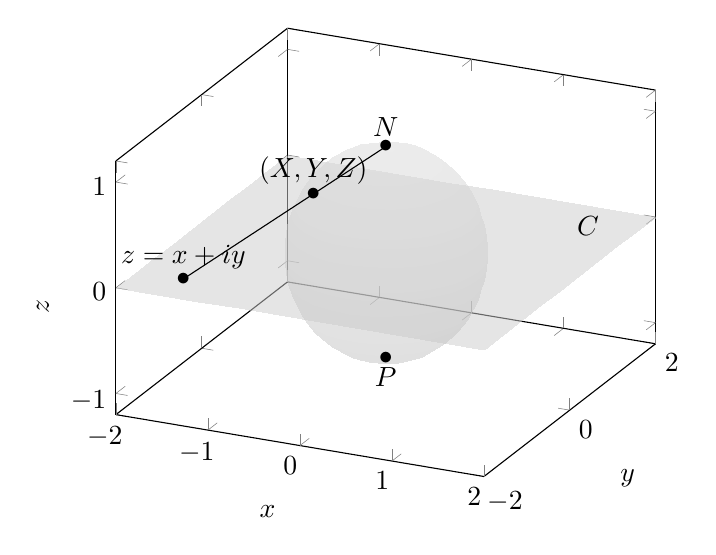
\begin{tikzpicture}\begin{axis}[xlabel=$x$,ylabel=$y$,zlabel=$z$,colormap={gray}{color=(gray!50!white) color=(gray!30!white)},z buffer=sort,shader=interp,fill opacity=.5,text opacity=1]
    \path[name path=l](0,0,1)--(-1.5,-1.5,0);
    \addplot3[name path=s,opacity=0,domain=0:.8,samples=30]({(1-x^2)^(1/2)*cos(225)},{(1-x^2)^(1/2)*sin(225)},{x});
    \path[name intersections={of=l and s}];

    \addplot3[domain=-2:2,y domain=-2:2,samples=10,surf](x,y,0);
    \addplot3[domain=-1:1,y domain=0:360,samples=20,samples y=30,surf]({(1-x^2)^(1/2)*cos(y)},{(1-x^2)^(1/2)*sin(y)},{x});
    \draw(0,0,1)node{$\bullet$}node[above]{$N$}--(intersection-1)node{$\bullet$}node[above]{$(X,Y,Z)$}--(-1.5,-1.5,0)node{$\bullet$}node[above]{$z=x+iy$};
    \draw(0,0,-1)node{$\bullet$}node[below]{$P$};
    \draw(1.5,1.5,0)node{$C$};
\end{axis}\end{tikzpicture}\end{document}